\documentclass[
    table,
    12pt,
    oneside,
    a4paper,
    english
]{book}

\PassOptionsToPackage{dvipsnames}{xcolor} % colori PDF/A

\usepackage{colorprofiles}
% PDF/A
% validate in https://www.pdf-online.com/osa/validate.aspx
\usepackage[a-1a,mathxmp]{pdfx}[2018/12/22]
\usepackage[T1]{fontenc}
\usepackage[utf8]{inputenc}
\usepackage[english]{babel}
\usepackage{bookmark}
\usepackage{caption}
\usepackage{comment}
\usepackage{chngpage, calc} % centra il frontespizio
\usepackage{emptypage} % pagine vuote senza testatina e piede di pagina
\usepackage{epigraph} % per epigrafi
\usepackage{indentfirst} % rientra il primo paragrafo di ogni sezione
\usepackage{graphicx} % immagini
\usepackage{mparhack,relsize}  % finezze tipografiche
\usepackage{nameref} % visualizza nome dei riferimenti
\usepackage[font=small]{quoting} % citazioni
\usepackage{subfig} % sottofigure, sottotabelle
\usepackage[italian]{varioref} % riferimenti completi della pagina
\usepackage{longtable} % tabelle su più pagine
\usepackage[toc, acronym]{glossaries}
\usepackage[backend=biber, backref, style=numeric]{biblatex}
\usepackage{lmodern}
\usepackage[top=2.75cm, bottom=2.75cm, right=3cm, left=3.75cm]{geometry} % 1in+17pt+0.6cm
\usepackage{fancyhdr}
\usepackage{lipsum}
\usepackage{setspace}
\usepackage{titlesec}
\usepackage{hyperref}
\usepackage[dvipsnames,hyperref=false]{xcolor}
\usepackage[normalem]{ulem}
\usepackage{sectsty}
\usepackage{sectsty} % gestisce i font di capitoli e sezioni
\usepackage{csquotes} % gestisce automaticamente i caratteri (")
\usepackage{etoolbox}
\usepackage[bottom]{footmisc}
\usepackage{zref-totpages}
% Load variables
\newcommand{\myUni}{University of Padua}
\newcommand{\myDepartment}{Department of Mathematics ``Tullio Levi-Civita''}
\newcommand{\myFaculty}{Master Degree in Computer Science}
\newcommand{\myTitle}{Lorem ipsum dolor sit amet, consectetur adipisci elit.}
\newcommand{\myDegree}{Master's Thesis}
\newcommand{\profTitle}{Prof.}
\newcommand{\myProf}{Ombretta Gaggi}
\newcommand{\graduateTitle}{Candidate}
\newcommand{\myName}{Gabriel Rovesti}
\newcommand{\myStudentID}{ID Number: 2103389}
\newcommand{\myAA}{2024-2025}
\newcommand{\myLocation}{Padova}
\newcommand{\myTime}{July 2025}
% Acronyms
\newacronym{ui}{UI}{User Interface}
\newacronym{ux}{UX}{User Experience}

% Glossary
\newglossaryentry{uig}{
    name={UI},
    text={User Interface},
    sort=ui,
    description={The User Interface refers to the space where interactions between humans and machines occur. It includes the design and arrangement of graphical elements (such as buttons, icons, and menus) that enable users to interact with software or hardware systems. The goal of a UI is to make the user's interaction simple and efficient in accomplishing tasks within a system.}
}

\newglossaryentry{uxg}{
    name={UX},
    text={User Experience},
    sort=ux,
    description={User Experience encompasses the overall experience a user has while interacting with a product or service. It includes not only usability and interface design but also the emotional response, satisfaction, and ease of use a person feels while using a system. UX design focuses on optimizing a product’s interaction to provide meaningful and relevant experiences to users, ensuring that the system is intuitive, efficient, and enjoyable to use.}
}

% Define custom colors
\definecolor{hyperColor}{HTML}{0B3EE3}
\definecolor{tableGray}{HTML}{F5F5F7}
\definecolor{veryPeri}{HTML}{6667ab}

% Set line height
\linespread{1.5}

% Custom hyphenation rules
\hyphenation {
    data-base
    al-go-rithms
    soft-ware
}

\begin{filecontents*}{\jobname.xmpdata}
  \Title{Lorem Ipsum}
  \Author{Gabriel Rovesti} 
  \Language{it-IT}
  \Subject{Lorem ipsum}
  \Keywords{X \sep Y \sep Zero Knowledge Proof (ZKP) \sep Z}
\end{filecontents*} 

% Images path
\graphicspath{{img/}}

% Force page color, as some editors set a grayish color as default
\pagecolor{white}

% Better spacing for footnotes
\setlength{\skip\footins}{5mm}
\setlength{\footnotesep}{5mm}

\setlength{\headheight}{14.5pt}
\addtolength{\topmargin}{-2.45pt}

% Add a subscript G to a glossary entry
\newcommand{\glox}{\textsubscript{\textbf{\textit{G}}}}

% Improvements the paragraph command
\titleformat{\paragraph}
{\normalfont\normalsize\bfseries}{\theparagraph}{1em}{}
\titlespacing*{\paragraph}
{0pt}{3.25ex plus 1ex minus .2ex}{1.5ex plus .2ex}

% Apply fancy styling to pages
\pagestyle{fancy}
\fancyhf{}
\fancyhead[L]{\leftmark} % Places Chapter N. Chatper title on the top left
\fancyfoot[C]{\thepage} % Page number in the center of the footer

% Adds a blank page while increasing the page number
\newcommand\blankpage{ 
\clearpage
    \begingroup
    \null
    \thispagestyle{empty}
    \hypersetup{pageanchor=false}
    \clearpage
\endgroup
}

% Adds a blank page while increasing the page number
\newcommand\blankpagewithnumber{ 
  \clearpage
  \thispagestyle{plain} % Use plain page style to keep the page number
  \null
  \clearpage
}

% Increase page numbering
\newcommand\increasepagenumbering{
    \addtocounter{page}{+1}
}

% Make glossaries and bibliography
\makeglossaries
% Redefine the format for the glossary entries to be italic
\renewcommand*{\glstextformat}[1]{\textit{#1}\glox}
\glsaddall

\bibliography{references/bibliography}
\defbibheading{bibliography} {
    \cleardoublepage
    \phantomsection
    \addcontentsline{toc}{chapter}{\bibname}
    \chapter*{\bibname\markboth{\bibname}{\bibname}}
}

% Set up hyperlinks
\hypersetup{
    colorlinks=true,
    linktocpage=true,
    pdfstartpage=1,
    pdfstartview=,
    breaklinks=true,
    pdfpagemode=UseNone,
    pageanchor=true,
    pdfpagemode=UseOutlines,
    plainpages=false,
    bookmarksnumbered,
    bookmarksopen=true,
    bookmarksopenlevel=1,
    hypertexnames=true,
    pdfhighlight=/O,
    allcolors = hyperColor
}

% Set up captions
\captionsetup{
    tableposition=top,
    figureposition=bottom,
    font=small,
    format=hang,
    labelfont=bf
}

\date{}

\hypersetup{pdfstartview=}
\begin{document}
    \frontmatter
    \begin{titlepage}
    \begin{center}
        \begin{Large}
            \textbf{\myUni}\\
        \end{Large}

        \vspace{5pt}

        \begin{large}
            \textsc{\myDepartment}\\
        \end{large}

        \vspace{5pt}

        \begin{large}
            \textsc{\myFaculty}\\
        \end{large}

        \vspace{25pt}
        
        \begin{figure}[htbp]
            \centering
            
\includegraphics[alt={Emblema dell'Università degli Studi di Padova}, height=6cm]{img/logo_unipd.jpeg}
        \end{figure}

        
        \begin{Large}
            \textbf{\myTitle}\\
        \end{Large}

        \vspace{5pt}

        \begin{large}
            \textit{\myDegree}\\
        \end{large}

        \vspace{50pt}
        
        \begin{normalsize}
            \begin{flushleft}
                \textit{Supervisor}\\
                \profTitle\ \myProf \\
                \textit{Co-supervisor}\\
                \profTitle\ {Catia Prandi}
            \end{flushleft}

            \vspace{-48pt}
            
            \begin{flushright}
                \textit{\graduateTitle}\\
                \myName\\
                \myStudentID
            \end{flushright}
        \end{normalsize}

        \vspace*{\fill}
        
        \line(1, 0){338} \\
        \begin{normalsize}
            \textsc{Academic Year \myAA}
        \end{normalsize}
    \end{center}
\end{titlepage}

    \increasepagenumbering % increase the page numbrering by 1, in order to cout the frontispiece
    \clearpage
\phantomsection
\thispagestyle{empty}
\hfill
\vfill

{\small\noindent\textcopyright\ \myName, \myTime. All rights reserved. \myDegree: ``\textit{\myTitle}'', \myUni, \myDepartment.}
    \cleardoublepage
\phantomsection
\pdfbookmark{Acknowledgements}{Acknowledgements}

\begin{flushright}{
    \slshape
    ``We don't read and write poetry because it's cute. We read and write poetry because we are members of the human race. And the human race is filled with passion. And medicine, law, business, engineering, these are noble pursuits and necessary to sustain life. But poetry, beauty, romance, love, these are what we stay alive for.''} \\
    \medskip
    --- N.H. Kleinbaum, Dead Poets Society
\end{flushright}

\begingroup
\let\clearpage\relax
\let\cleardoublepage\relax
\let\cleardoublepage\relax

\chapter*{Acknowledgements}

\noindent First and foremost, I would like to express my gratitude to Prof. Gaggi, given her support throughout two paths of thesis, both in bachelor and master degrees, for valuable knowledge and support throughout these academic years, both humanly and academically. 

\vspace{0.35cm}

\noindent I would like to thank my mom, the only person who supported me practically throughout these years and gave me many life lessons, maybe not in the right way, but her love was always present for me. For the same reason, my life has been very dense of things, but I promised myself I would have always been able to make it. And I did it always on my own, in ways I would have never imagined since I had no guidance, but I was always everyone guidance. Not arrogance, simply human nature. I hope after this huge step to conquer the long awaited peace of spirit and soul. 

\vspace{0.35cm}

\noindent A special thank you to the few real friends I have (first of all Matilde), because they helped me do many things up until now and I would not live a day without them.

\vspace{0.75cm}

\noindent{\myLocation, \myTime}
\hfill \textit{\myName}

\endgroup

    \cleardoublepage
\phantomsection
\pdfbookmark{Abstract}{Abstract}
\begingroup
\let\clearpage\relax
\let\cleardoublepage\relax
\chapter*{Abstract}
This thesis presents a systematic comparative analysis of accessibility implementation approaches in mobile application development frameworks, specifically React Native and Flutter. Building upon previous research focused on Flutter's accessibility capabilities, this study extends the investigation to provide a comprehensive examination of how both frameworks enable developers to create accessible mobile user interfaces.

The research methodology encompasses the development of \textit{AccessibleHub}—an educational toolkit application that serves as both a research vehicle and practical resource for developers. Through this implementation, the study identifies specific patterns, similarities, differences, and potential improvements in accessibility implementation between the frameworks. The analysis examines implementation complexity, developer experience, and compliance with Web Content Accessibility Guidelines (WCAG) 2.2 standards, providing quantitative metrics for framework comparison. \\

A core contribution of this work is the translation of abstract accessibility guidelines into concrete implementation patterns, bridging the gap between theoretical requirements and practical code. The research demonstrates that while both frameworks can achieve equivalent accessibility outcomes, they differ significantly in their architectural approaches and implementation overhead. React Native employs a property-based model that typically requires less code but offers less explicit semantic control, while Flutter's widget-based semantic system provides more granular accessibility management at the cost of increased implementation complexity. 

\pagebreak

Accessibility represents not merely a compliance requirement but a fundamental aspect of both user experience and developer mindset. By expanding product usability across diverse user populations regardless of capabilities, properly implemented accessibility features ensure seamless interaction across components and devices. This research provides evidence-based guidance for framework selection and implementation strategies, contributing to the advancement of accessible mobile application development as technology continues to evolve.
\endgroup
\vfill
    \cleardoublepage
\renewcommand{\contentsname}{Table of contents}
\pdfbookmark{\contentsname}{tableofcontents}
\setcounter{secnumdepth}{5}
\setcounter{tocdepth}{5}     
\tableofcontents
\clearpage
\begingroup
    \let\clearpage\relax
    \let\cleardoublepage\relax
    \let\cleardoublepage\relax
    % Figures list
    \phantomsection
    \renewcommand{\listfigurename}{List of figures}
    \pdfbookmark{\listfigurename}{lof}
    \listoffigures
    \vspace*{8ex}
    % Tables list
    \phantomsection
    \renewcommand{\listtablename}{List of tables}
    \pdfbookmark{\listtablename}{lot}
    \listoftables
    % Listings list
    \phantomsection
    \addcontentsline{toc}{chapter}{\lstlistlistingname}
    \lstlistoflistings
\endgroup
\cleardoublepage
    \printglossary[type=\acronymtype, title=Acronims and abbreviations, toctitle=Acronims and abbreviations]
    \printglossary[type=main, title=Glossary, toctitle=Glossary]
    \blankpage % example of a blank page that also increases the page couter by 1

    \mainmatter
    \chapter{Introduction}
\label{chap:intro}

\chapterintroline{
    This chapter explores the fundamental aspects of mobile accessibility, examining how different user capabilities, device interactions, and usage contexts shape the landscape of accessible mobile development. 
}

\section{Mobile accessibility: context \& foundations}
\label{chap:intro-background}

In an era where digital technology permeates every aspect of our lives, mobile devices have emerged as the primary gateway to the digital world, allowing a lot of new people to be connected at any given time, no matter the condition. An estimated number of circa 7 billions \cite{article:number-of-users}, representing a dramatic increase from just one billion users in 2013, is currently using mobile devices and exploiting the possibilities they offer on an everyday basis. This explosive growth has not only changed how we communicate and access information but has also created a massive market for different needs and introduced new categories of users, with different habits and cultures into a truly global market.

As mobile applications become increasingly central to daily life, ensuring their accessibility to all users, regardless of their abilities or disabilities, has become a critical imperative, since not only technology should be able to connect, but also to unite seamlessly people with different capabilities. Accessibility refers to the design and development practices enabling all users, regardless of their abilities or disabilities, to perceive, understand and navigate with digital content effectively. Not only the quantity of media increased, but also the quantity of different media which allow to access information definitely increased; finding appropriate measurements to establish a good level of understanding and usability is important and finding appropriate levels of measurements is non-trivial. \\

An estimated portion of over one billion people lives globally with some forms of disability \cite{article:who-disability}. Inaccessible mobile applications can, therefore, present considerable barriers to participation in that large and growing part of modern life that involves education, employment, social interaction, and even basic services. Accessibility is not about a majority giving special dispensation to a minority but rather about providing equal access and opportunities to very big and diverse user bases.

This encompasses a wide range of considerations to be made on the actual products design and the user classes, including but not limited to:
\begin{enumerate}
    \item \textit{Visual accessibility}: supporting users who have a visual impairment or low vision, requiring alternative description and screen readers support;

    \item \textit{Auditory accessibility}: providing alternatives for users who have a hearing impairment or hard of hearing, offering clear controls and alternative  visuals for audio content, ensuring compatibility with assistive devices and giving feedback to specific actions done by users;

    \item \textit{Motor accessibility}: accommodating users with limited dexterity or mobility, providing alternative input navigation, create a design so to help avoiding complex gestures, customize the interactions and gestures, reducing precision and accommodating errors;

    \item \textit{Cognitive accessibility}: ensuring content is understandable for users with different cognitive abilities. This includes having consistent and predictable navigation, using visual aids to help users stay focused, and making sure all parts of the interface are easy to understand, providing a language which is clear, concise and straightforward.
    
\end{enumerate}

In the mobile environment, such considerations is important, since there is a complex web of interactions to be considered, mainly focusing on two aspects:

\begin{enumerate}
    \item \textit{Device diversity and integration} - accommodating different gestures, interfaces and interaction modalities
        \begin{itemize}
            \item Standard mobile devices (smartphones, tablets);
            \item Emerging device formats (foldables, dual-screen devices);
            \item Wearable technology (smartwatches, fitness trackers);
            \item Embedded systems (vehicle interfaces, smart home controls);
            \item IoT devices with mobile interfaces.
        \end{itemize}
    \item \textit{Usage context variations} - may influence the overload of information and the cognitive load perceived by the user
        \begin{itemize}
            \item Environmental conditions (lighting, noise, movement);
            \item User posture and mobility situations;
            \item Attention availability and cognitive load;
            \item Physical constraints and limitations;
            \item Social and cultural contexts.
        \end{itemize}
\end{enumerate}

These considerations are important since they impact how accessibility features should go above and beyond, carefully considering how the interaction in mobile devices is used. Mobile devices offer multiple interaction modalities, which must be considered for an inclusive design:

\begin{itemize}
    \item \textit{Touch-based interactions}: here, traditional interactions present specific challenges and opportunities for accessibility: actions like tapping (selection/activation), double tapping (confirmation/secondary actions), long pressing (contextual menus/additional options), swiping (navigation/list scrolling) and pinching (zoom control) are used. These gestures may need alternatives regarding timing in long presses, touch stabilization and increased touch target sizes, since they can be also combined with multiple patterns e.g. multi-finger gestures and edge swipes;
    
    \item \textit{Voice control and speech input}: navigation commands and action triggers can be activated giving directions (e.g. "go back", "scroll down"), inputting text thorough dictation, while giving auditory feedback and interactions vocally;
    
    \item \textit{Motion and sensor-based input}: modern devices offer various sensor-based interaction methods, like tilting controls for navigation, shaking gestures for specific actions, orientation changes for layout adaptation, using proximity sensors to detect gestures without touch;
    
    \item \textit{Switch access and external devices}: providing support for alternative input methods is crucial, providing physical single or multiple switch support, sequential focus navigation and customizable timing controls. Some users might find useful to have external input devices like keyboards, specialized controllers, Braille displays, but also help from custom assistive devices;
    
    \item \textit{Haptic feedback}: tactile feedback provides important interaction cues, on actions confirmation, error notifications and context-sensitive responses, e.g. force-touch interactions and pressure-based controls.
\end{itemize}

It's useful to analyze such commands since the focus would be describing how to address accessibility issues and have a complete focus on how a user would interact with an interface and a mobile device, since each interaction provides a different degree of complexity. Understanding built-in capabilities is crucial for developers working with cross-platform frameworks, as they must effectively bridge their applications with native features. These tools will be discussed from an high-level, so to describe their role and goals, among functionalities:

\begin{itemize}
    \item \textit{TalkBack for Android}: Google's screen reader provides comprehensive accessibility support through:
        \begin{itemize}
            \item Linear navigation mode that allows users to systematically explore screen content through swipe gestures, which replaces traditional mouse or direct touch interaction;
            \item Touch exploration mode allowing users to hear screen content by touching it and make navigation predictable and systematic;
            \item Custom gesture navigation system for efficient interface interaction;
            \item Customizable feedback settings for different user preferences;
            \item Integration with external Braille displays and keyboards (also with complementary services like \textit{BrailleBack});
            \item Support for different languages and speech rates
            \item Help in combination of \textit{Switch Access}, built-in feature to help users using switches instead of touch gestures.
        \end{itemize}
    
    \item \textit{VoiceOver for iOS}: Apple's integrated screen reader offers:
        \begin{itemize}
            \item Rotor control for customizable navigation options;
            \item Advanced gesture recognition system;
            \item Direct touch exploration of screen elements;
            \item Automatic language detection and switching;
            \item Comprehensive Braille support across multiple standards;
            \item Complete integration with \textit{Zoom}, a built-in screen magnifier present in iOS devices to zoom in on any part of the screen;
            \item Integrated with other a suite of other accessibility tools present in iOS devices, available to all users.
        \end{itemize}

    \item \textit{Select to Speak for Android}: A complementary feature that provides:
        \begin{itemize}
            \item On-demand reading of selected screen content;
            \item Visual highlighting of spoken text;
            \item Simple activation through dedicated gestures;
            \item Integration with system-wide accessibility settings.
        \end{itemize}
\end{itemize}

This thesis examines the implementation of accessibility support in two leading mobile development frameworks—Flutter and React Native—with particular attention to their integration with native accessibility features. The architectural approaches differ significantly: Flutter creates a structured accessibility tree that maps to native accessibility \acrshort{api}, while React Native establishes direct bindings to platform-specific accessibility features. This fundamental difference profoundly influences how developers must conceptualize and implement accessibility within their applications, a distinction that will be thoroughly explored throughout this work.

\section{Thesis structure}
\label{chap:intro-structure} 

In this subsection, a brief description of the rest of the thesis is given:

\begin{description}
    \item[{\hyperref[chap:accessibility]{The second chapter}}] presents a comprehensive literature review of mobile accessibility, examining specific guidelines for mobile applications including WCAG adaptations, platform-specific requirements for iOS and Android, regulatory frameworks, implementation considerations, and testing methodologies. This chapter establishes the theoretical foundation for understanding the current accessibility landscape;
    
    \item[{\hyperref[chap:accessibility-toolkit]{The third chapter}}] introduces the \textit{AccessibleHub} project—a React Native application serving as an interactive guide for implementing accessibility features in mobile applications. This chapter details the architectural design, implementation patterns, and educational framework underpinning this novel approach to mobile accessibility. \textit{AccessibleHub} methodically addresses the challenges developers face when translating abstract WCAG guidelines into practical implementations, extending previous research to provide a developer-centric toolkit that analyzes how React Native and Flutter handle accessibility through interactive examples and component-level guidance;
    
    \item[{\hyperref[chap:accessibility-implementation]{The fourth chapter}}] provides a detailed analysis of WCAG guideline implementation across frameworks, examining implementation complexity, performance implications, developer experience, and testing methodologies. This chapter offers comparative insights into accessibility implementation between React Native and Flutter, identifying best practices, common pitfalls, and optimization strategies;
    
    \item[{\hyperref[chap:conclusions]{The final chapter}}] synthesizes research findings into actionable guidance for developers and project stakeholders. The chapter discusses implications for mobile developers, including framework-specific optimization approaches and evidence-based implementation priorities. It acknowledges methodological, technical, and scope limitations of the research, including component selection constraints and framework version dependencies.
\end{description}

To enhance readability and ensure clarity, this thesis adopts the following typographical conventions:
\begin{itemize}
    \item Acronyms, abbreviations, and technical terms are defined in the glossary;
    \item First occurrences of glossary terms use the format: \gls{wcagg};
    \item Foreign language terms and technical jargon appear in \textit{italic};
    \item Code examples use \texttt{monospace} formatting when discussed within text or proper custom coloring form to be used within the rest of sections.
\end{itemize}

\newpage
    % \chapter{Processi e metodologie}
\label{chap:processi-metodologie}

Lorem ipsum dolor sit amet, consectetuer adipiscing elit. Aenean commodo ligula eget dolor. Aenean massa. Cum sociis natoque\footnote{\cite{site:agile-manifesto}} penatibus et magnis dis parturient montes, nascetur ridiculus mus. Donec quam felis, ultricies nec\footnote{\cite{article:spooky}}, pellentesque eu, pretium quis, sem.

\begin{figure}[H]
    \centering
    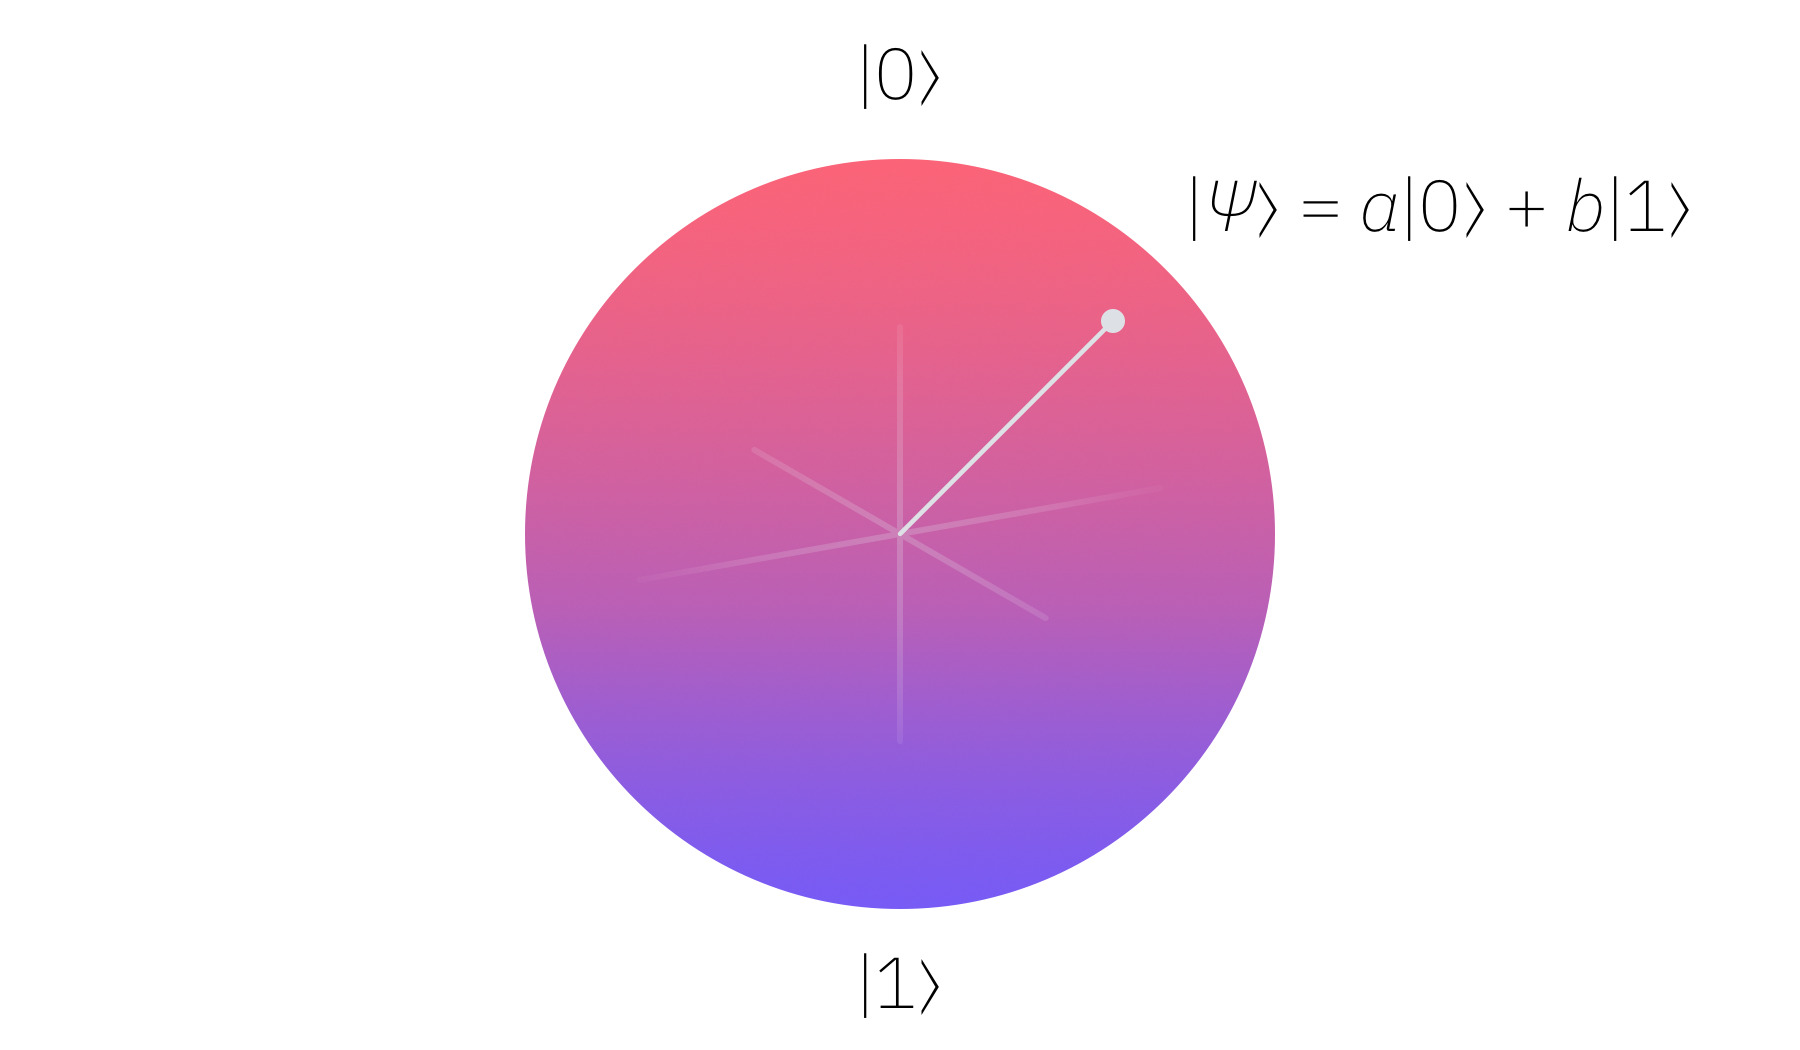
\includegraphics[alt={Testo alternativo dell'immagine}, height=5cm]{img/qubit.jpeg}
    \description[Rappresenzazione Qubit]{Long description}
    \caption{Lorem}
    \label{fig:qubit}
\end{figure}
\lipsum[1]

\section{Processo sviluppo prodotto}
\lipsum[1-2]

\begin{listing}[H]
\begin{minted}{c}
#include <stdio.h>
int main() {
    print("Hello, world!");
    return 0;
}
\end{minted}
\caption{Example of code}
\label{listing:b}
\end{listing}

Lorem ipsum:
\begin{listing}[H]
\begin{minted}{c}
#include <stdio.h>
int main() {
    print("Hello, world!");
    return 0;
}
\end{minted}
\caption{Example of code}
\label{listing:b-2}
\end{listing}

Lorem ipsum:
\begin{listing}[H]
\begin{minted}{c}
#include <stdio.h>
int main() {
    print("Hello, world!");
    return 0;
}
\end{minted}
\caption{Example of code}
\label{listing:b-3}
\end{listing}

\newpage
    % \chapter{Descrizione dello stage}
\label{chap:descrizione-stage}

\section{Introduzione al progetto}
\begin{figure}[H] 
    \centering 
    
\includegraphics[alt={Testo alternativo dell'immagine}, width=0.5\columnwidth]{img/pk_estate.jpeg}
    \caption{Caption}
    \label{fig:pk_estate}
\end{figure}
\lipsum[1]

\section{Analisi preventiva dei rischi}

Durante la fase di analisi iniziale sono stati individuati alcuni possibili rischi a cui si potrà andare incontro.
Si è quindi proceduto a elaborare delle possibili soluzioni per far fronte a tali rischi.

\begin{risk}{Performance del simulatore hardware}
    \riskdescription{le performance del simulatore hardware e la comunicazione con questo potrebbero risultare lenti o non abbastanza buoni da causare il fallimento dei test}
    \risksolution{coinvolgimento del responsabile a capo del progetto relativo il simulatore hardware}
    \label{risk:hardware-simulator} 
\end{risk}

\section{Requisiti e obiettivi}

\begin{center}
    \rowcolors{1}{}{tableGray}
    \begin{longtable}{|p{2.25cm}|p{7.75cm}|p{2.25cm}|}
    \hline
    \multicolumn{1}{|c|}{\textbf{A}} & \multicolumn{1}{c|}{\textbf{B}}\\ 
    \hline 
    \endfirsthead
    \rowcolor{white}
    \multicolumn{3}{c}{{\bfseries \tablename\ \thetable{} -- Continuo della tabella}}\\
    \hline
    \multicolumn{1}{|c|}{\textbf{A}} & \multicolumn{1}{c|}{B}\\ \hline 
    \endhead
    \hline
    \rowcolor{white}
    \multicolumn{3}{|r|}{{Continua nella prossima pagina...}}\\
    \hline
    \endfoot
    \endlastfoot 
    
    AA & BB \\
    \hline
    AA & BB \\
    \hline
    AA & BB \\
    \hline
    AA & BB \\
    \hline
    \hiderowcolors
    \caption{Lorem.}
    \label{tab:requisiti_obbiettivi}
    \end{longtable}
\end{center}

\section{Pianificazione}
\begin{figure}[H]
    \centering
    
\includegraphics[alt={Testo alternativo dell'immagine}, width=0.5\columnwidth]{img/pk_estate.jpeg}
    \caption{Caption}
    \label{fig:pk_estate_2}
\end{figure}
\lipsum[1]

\subsection{subsection}
\lipsum[1]

\subsubsection{subsubsection}
\lipsum[1]

\paragraph{paragraph}
\lipsum[1]

\newpage
    % \chapter{Analisi dei requisiti}
\label{chap:analisi-requisiti}

\section{Casi d'uso}
Per lo studio dei casi di utilizzo del prodotto sono stati creati dei diagrammi.
I diagrammi dei casi d'uso (in inglese \textit{Use Case Diagram}) sono diagrammi di tipo \gls{uml} dedicati alla descrizione delle funzioni o servizi offerti da un sistema, così come sono percepiti e utilizzati dagli attori che interagiscono col sistema stesso.
Essendo il progetto finalizzato alla creazione di un tool \gls{TermineSenzaAcronimo} per l'automazione di un processo, le interazioni da parte dell'utilizzatore devono essere ovviamente ridotte allo stretto necessario. Per questo motivo i diagrammi d'uso risultano semplici e in numero ridotto.

\begin{figure}[H]
    \vspace{2em}
    \centering
    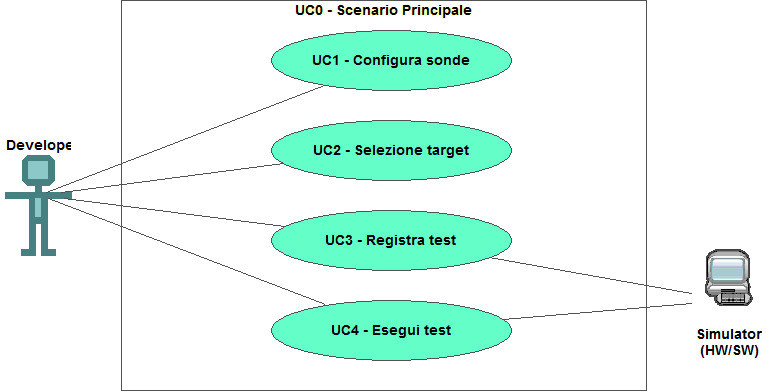
\includegraphics[alt={Testo alternativo dell'immagine}, width=0.75\columnwidth]{img/usecase/scenario-principale.jpeg}
    \caption{Use Case 0: Scenario principale}
    \label{fig:scenario_principale}
\end{figure}

\begin{usecase}{0}{Scenario principale}
    \usecaseactors{Sviluppatore applicativi.}
    \usecasepre{Lo sviluppatore è entrato nel plugin di simulazione all'interno dell'IDE.}
    \usecasedesc{La finestra di simulazione mette a disposizione i comandi per configurare, registrare o eseguire un test.}
    \usecasepost{Il sistema è pronto per permettere una nuova interazione.}
    \label{uc:uc_scenario_principale}
\end{usecase}

\begin{usecase}{1}{Gestione Utente}
    \usecaseactors{Amministratore, Utente Registrato.}
    \usecasepre{L'utente deve essere autenticato nel sistema.}
    \usecasedesc{L'utente può gestire le informazioni del proprio profilo.}
    \usecasepost{Le modifiche vengono salvate nel sistema.}
    \usecasealt{Se l'utente non è autenticato, visualizza un messaggio di errore.}
    \label{uc:uc_casi_uso}
\end{usecase}

\begin{usecase}{2}{Creazione Prodotto}
    \usecaseactors{Amministratore.}
    \usecasepre{L'amministratore ha effettuato l'accesso al sistema.}
    \usecasedesc{L'amministratore può aggiungere un nuovo prodotto al catalogo.}
    \usecasepost{Il nuovo prodotto viene aggiunto con successo.}
    \usecasealt{Se i campi obbligatori non sono compilati, visualizza un messaggio di errore.}
    \label{uc:uc_creazione_prodotto}
\end{usecase}

\section{Tracciamento dei requisiti}
Da un'attenta analisi dei requisiti e degli use case effettuata sul progetto è stata stilata la tabella che traccia i requisiti in rapporto agli use case.\\
Sono stati individuati diversi tipi di requisiti e si è quindi fatto utilizzo di un codice identificativo per distinguerli.\\
Il codice dei requisiti, dove ogni requisito è identificato con il carattere \textbf{R}, è così strutturato:
\begin{enumerate}
    \item[\textbf{F}:] Funzionale.
    \item[\textbf{Q}:] Qualitativo.
    \item[\textbf{V}:] Di vincolo.
    \item[\textbf{N}:] Obbligatorio (necessario).
    \item[\textbf{D}:] Desiderabile.
    \item[\textbf{Z}:] Opzionale.
\end{enumerate}

Nelle tabelle \ref{tab:requisiti_funzionali}, \ref{tab:requisiti_qualitativi} e \ref{tab:requisiti_vincolo} sono riassunti i requisiti e il loro tracciamento con gli use case delineati in fase di analisi.

\section{Tabelle dei requisiti}
\begin{center}
    \rowcolors{1}{}{tableGray}
    \begin{longtable}{|p{2.25cm}|p{7.75cm}|p{2.25cm}|}
    \hline
    %\rowcolor{hyperColor!5}
    \multicolumn{1}{|c|}{\textbf{Requisito}} & \multicolumn{1}{c|}{\textbf{Descrizione}} & \multicolumn{1}{c|}{\textbf{Use Case}}\\
    \hline 
    \endfirsthead
    \rowcolor{white}
    \multicolumn{3}{c}{{\bfseries \tablename\ \thetable{} -- Continuo della tabella}}\\
    \hline
    %\rowcolor{hyperColor!5}
    \multicolumn{1}{|c|}{\textbf{Requisito}} & \multicolumn{1}{c|}{\textbf{Descrizione}} & \multicolumn{1}{c|}{\textbf{Use Case}}\\
    \hline 
    \endhead
    \hline
    \rowcolor{white}
    \multicolumn{3}{|r|}{{Continua nella prossima pagina...}}\\
    \hline
    \endfoot
    \endlastfoot
    
    RFN-1 & L’interfaccia permette di configurare il tipo di sonde del test & UC1 \\
    \hline
    \hiderowcolors
    \caption{Tabella del tracciamento dei requisiti funzionali.}
    \label{tab:requisiti_funzionali}
    \end{longtable}
\end{center}

\begin{center}
    \rowcolors{1}{}{tableGray}
    \begin{longtable}{|p{2.25cm}|p{7.75cm}|p{2.25cm}|}
    \hline
    %\rowcolor{hyperColor!5}
    \multicolumn{1}{|c|}{\textbf{Requisito}} & \multicolumn{1}{c|}{\textbf{Descrizione}} & \multicolumn{1}{c|}{\textbf{Use Case}}\\
    \hline 
    \endfirsthead
    \rowcolor{white}
    \multicolumn{3}{c}{{\bfseries \tablename\ \thetable{} -- Continuo della tabella}}\\
    \hline
    %\rowcolor{hyperColor!5}
    \multicolumn{1}{|c|}{\textbf{Requisito}} & \multicolumn{1}{c|}{\textbf{Descrizione}} & \multicolumn{1}{c|}{\textbf{Use Case}}\\
    \hline 
    \endhead
    \hline
    \rowcolor{white}
    \multicolumn{3}{|r|}{{Continua nella prossima pagina...}}\\
    \hline
    %\caption{Tabella del tracciamento dei requisiti qualitativi.}
    \endfoot
    \endlastfoot
    
    RQD-1n & Le prestazioni del simulatore hardware deve garantire la giusta esecuzione dei test e non la generazione di falsi negativi & - \\
    \hline
    RQD-1n & Le prestazioni del simulatore hardware deve garantire la giusta esecuzione dei test e non la generazione di falsi negativi & - \\
    \hline
    RQD-1n & Le prestazioni del simulatore hardware deve garantire la giusta esecuzione dei test e non la generazione di falsi negativi & - \\
    \hline
    RQD-1n & Le prestazioni del simulatore hardware deve garantire la giusta esecuzione dei test e non la generazione di falsi negativi & - \\
    \hline
    RQD-1n & Le prestazioni del simulatore hardware deve garantire la giusta esecuzione dei test e non la generazione di falsi negativi & - \\
    \hline
    RQD-1n & Le prestazioni del simulatore hardware deve garantire la giusta esecuzione dei test e non la generazione di falsi negativi & - \\
    \hline
    \hiderowcolors
    \caption{Tabella del tracciamento dei requisiti qualitativi.}
    \label{tab:requisiti_qualitativi}
    \end{longtable}
\end{center}

\begin{center}
    \rowcolors{1}{}{tableGray}
    \begin{longtable}{|p{2.25cm}|p{7.75cm}|p{2.25cm}|}
    \hline
    %\rowcolor{hyperColor!5}
    \multicolumn{1}{|c|}{\textbf{Requisito}} & \multicolumn{1}{c|}{\textbf{Descrizione}} & \multicolumn{1}{c|}{\textbf{Use Case}}\\
    \hline 
    \endfirsthead
    \rowcolor{white}
    \multicolumn{3}{c}{{\bfseries \tablename\ \thetable{} -- Continuo della tabella}}\\
    \hline
    %\rowcolor{hyperColor!5}
    \multicolumn{1}{|c|}{\textbf{Requisito}} & \multicolumn{1}{c|}{\textbf{Descrizione}} & \multicolumn{1}{c|}{\textbf{Use Case}}\\
    \hline 
    \endhead
    \hline
    \rowcolor{white}
    \multicolumn{3}{|r|}{{Continua nella prossima pagina...}}\\
    \hline
    \endfoot
    \endlastfoot
    
    RVO-1 & La libreria per l'esecuzione dei test automatici deve essere riutilizzabile & - \\
    \hline
    \hiderowcolors
    \caption{Tabella del tracciamento dei requisiti di vincolo.}
    \label{tab:requisiti_vincolo}
    \end{longtable}
\end{center}

\newpage
    % \chapter{Progettazione e codifica}
\label{chap:progettazione-codifica}
Breve introduzione al capitolo

\section{Tecnologie e strumenti}
\label{sec:tecnologie-strumenti}
Di seguito viene data una panoramica delle tecnologie e strumenti utilizzati.

\subsection*{Tecnologia 1}
Descrizione Tecnologia 1.

\subsection*{Tecnologia 2}
Descrizione Tecnologia 2

\section{Ciclo di vita del software}
\label{sec:ciclo-vita-software}

\section{Progettazione}
\label{sec:progettazione}

\subsection{Namespace 1}
Descrizione namespace 1.

\section{Design Pattern utilizzati}

\section{Codifica}
Blocco di codice in C
\begin{listing}[H]
\begin{minted}{c}
#include <stdio.h>
int main() {
    print("Hello, world!");
    return 0;
}
\end{minted}
\caption{Example of code}
\label{listing:c}
\end{listing}

\newpage
    % \chapter{Verifica e validazione}
\label{chap:verifica-validazione}

\begin{figure}[H]
    \centering
    
\includegraphics[alt={Testo alternativo dell'immagine}, width=1\columnwidth]{img/quantum_superposition.jpeg}
    \caption{Lorem}
    \label{fig:enter-label}
\end{figure}

\lipsum[1-2]

% Esempio di come importare un file contenente codice
Lorem ipsum:
\begin{listing}[H]
\inputminted{python}{code/example.py}
\caption{Fibonacci recursive}
\label{listing:py_fibo}
\end{listing}

\lipsum[1]

\newpage
    % \chapter{Conclusions}
\label{chap:conclusions}

\section{Consuntivo finale}
Esempio di aggiunta di un termine con glossario e acronimo:\\
Lorem \gls{sdk} ispum dolor.

Nel successivo utilizzo, apparirà solo l'acronimo:\\
Lorem \gls{sdk}.

Nel caso si voglia invece mettere solo il termine per esteso, si può usare:\\
Lorem \gls{sdkg}.

\section{Raggiungimento degli obiettivi}
Esempio di termine con solo acronimo\\
Lorem \gls{tsa}, ipsum dolor sit amet

termine costruito senza acronimo:
Lorem \gls{TermineSenzaAcronimo}, ipsum dolor sit amet

\section{Conoscenze acquisite}
Lorem Ipsum dolor Lorem \gls{api}

Lorem Ipsum dolor Lorem \gls{apig}

Si può consultare il file \textit{glossary\_acronyms.tex} per alcuni esempi.

\section{Valutazione personale}


\section{Valutazione personale}


\newpage

    \pagenumbering{roman}
    \backmatter
    \chapter{Bibliography}
\label{cap:bibliography}

\nocite{*}

% Books bibliography
\printbibliography[heading=subbibliography, title={Books}, type=book]

% Articles bibliography
\printbibliography[heading=subbibliography, title={Articles and papers}, type=article]

% Websites bibliography
\printbibliography[heading=subbibliography, title={Sites}, type=online]

\end{document}